\documentclass[a4paper,10pt]{article}
\usepackage[utf8]{inputenc}
\usepackage{amsmath}
\usepackage{graphicx}

%opening
\title{Methods used}
\author{Bram van Es \& Sebastiaan Jong}

\begin{document}


\begin{abstract}

\end{abstract}


% Description of what is done
  % Detailed description of array normalization and batch correction strategy
  % Detailed description of procedures
  % Potential literature references
  % Flow charts
  % Thresholds/cut-offs
  % Iterations
  % Scripts (github), some journals require scripts
% In between results
  % Description of results obtained using your strategy and validation.
  % Plots/tables/text containing information of why this is a valid approach, for multiple steps
  % Rational behind the idea, prove of correctness
% Prediction of HR/NHR for ALL10
% Prediction of HR/NHR for Cohort1


\section{Pre-processing}

\subsection{Cohort-bias removal}
%
For the cohort-bias removal we apply a genome-wise Location and scale (L/S) adjustment per cohort.
Using a normalisation per cohort guarantees that the features have the same bounds 
over the cohorts and that the means are similar. The caveat of this approach is that we asume 
that the genome expression measurements are independent and we have no outliers.
%
The standard normalisation transforms the genome expression values $\mathbf{x}$ per genome as follows
\begin{equation}
  \mathbf{x}^* = \frac{\mathbf{x} - \overline{\mathbf{x}}}{\sigma},
\end{equation}
%
where $\mathbf{x}$ is the genome expression vector for some genome over all samples. 
This centers the mean and normalises the  expression values with the standard deviation. 
To limit the influence of outliers we can center the median and use the interquantile range (IQR)
for the scaling, i.e.
%
\begin{equation}
  \mathbf{x}^* = \frac{\mathbf{x} - median\left({\mathbf{x}}\right)}{IQR},
\end{equation}
%
%To ensure similar bounds we can then scale the values by largest absolute value per genome vector, i.e.
%\begin{equation}
%  \mathbf{x}^* = \frac{\mathbf{x}}{\max{(\mathbf{x})}}.
%\end{equation}
%
To demonstrate the effect of these transformations with regard to cohort bias we take two genomes, one with high and one with low variance
over the classifications. \\ \\
%
\begin{figure}[htp]
\centering
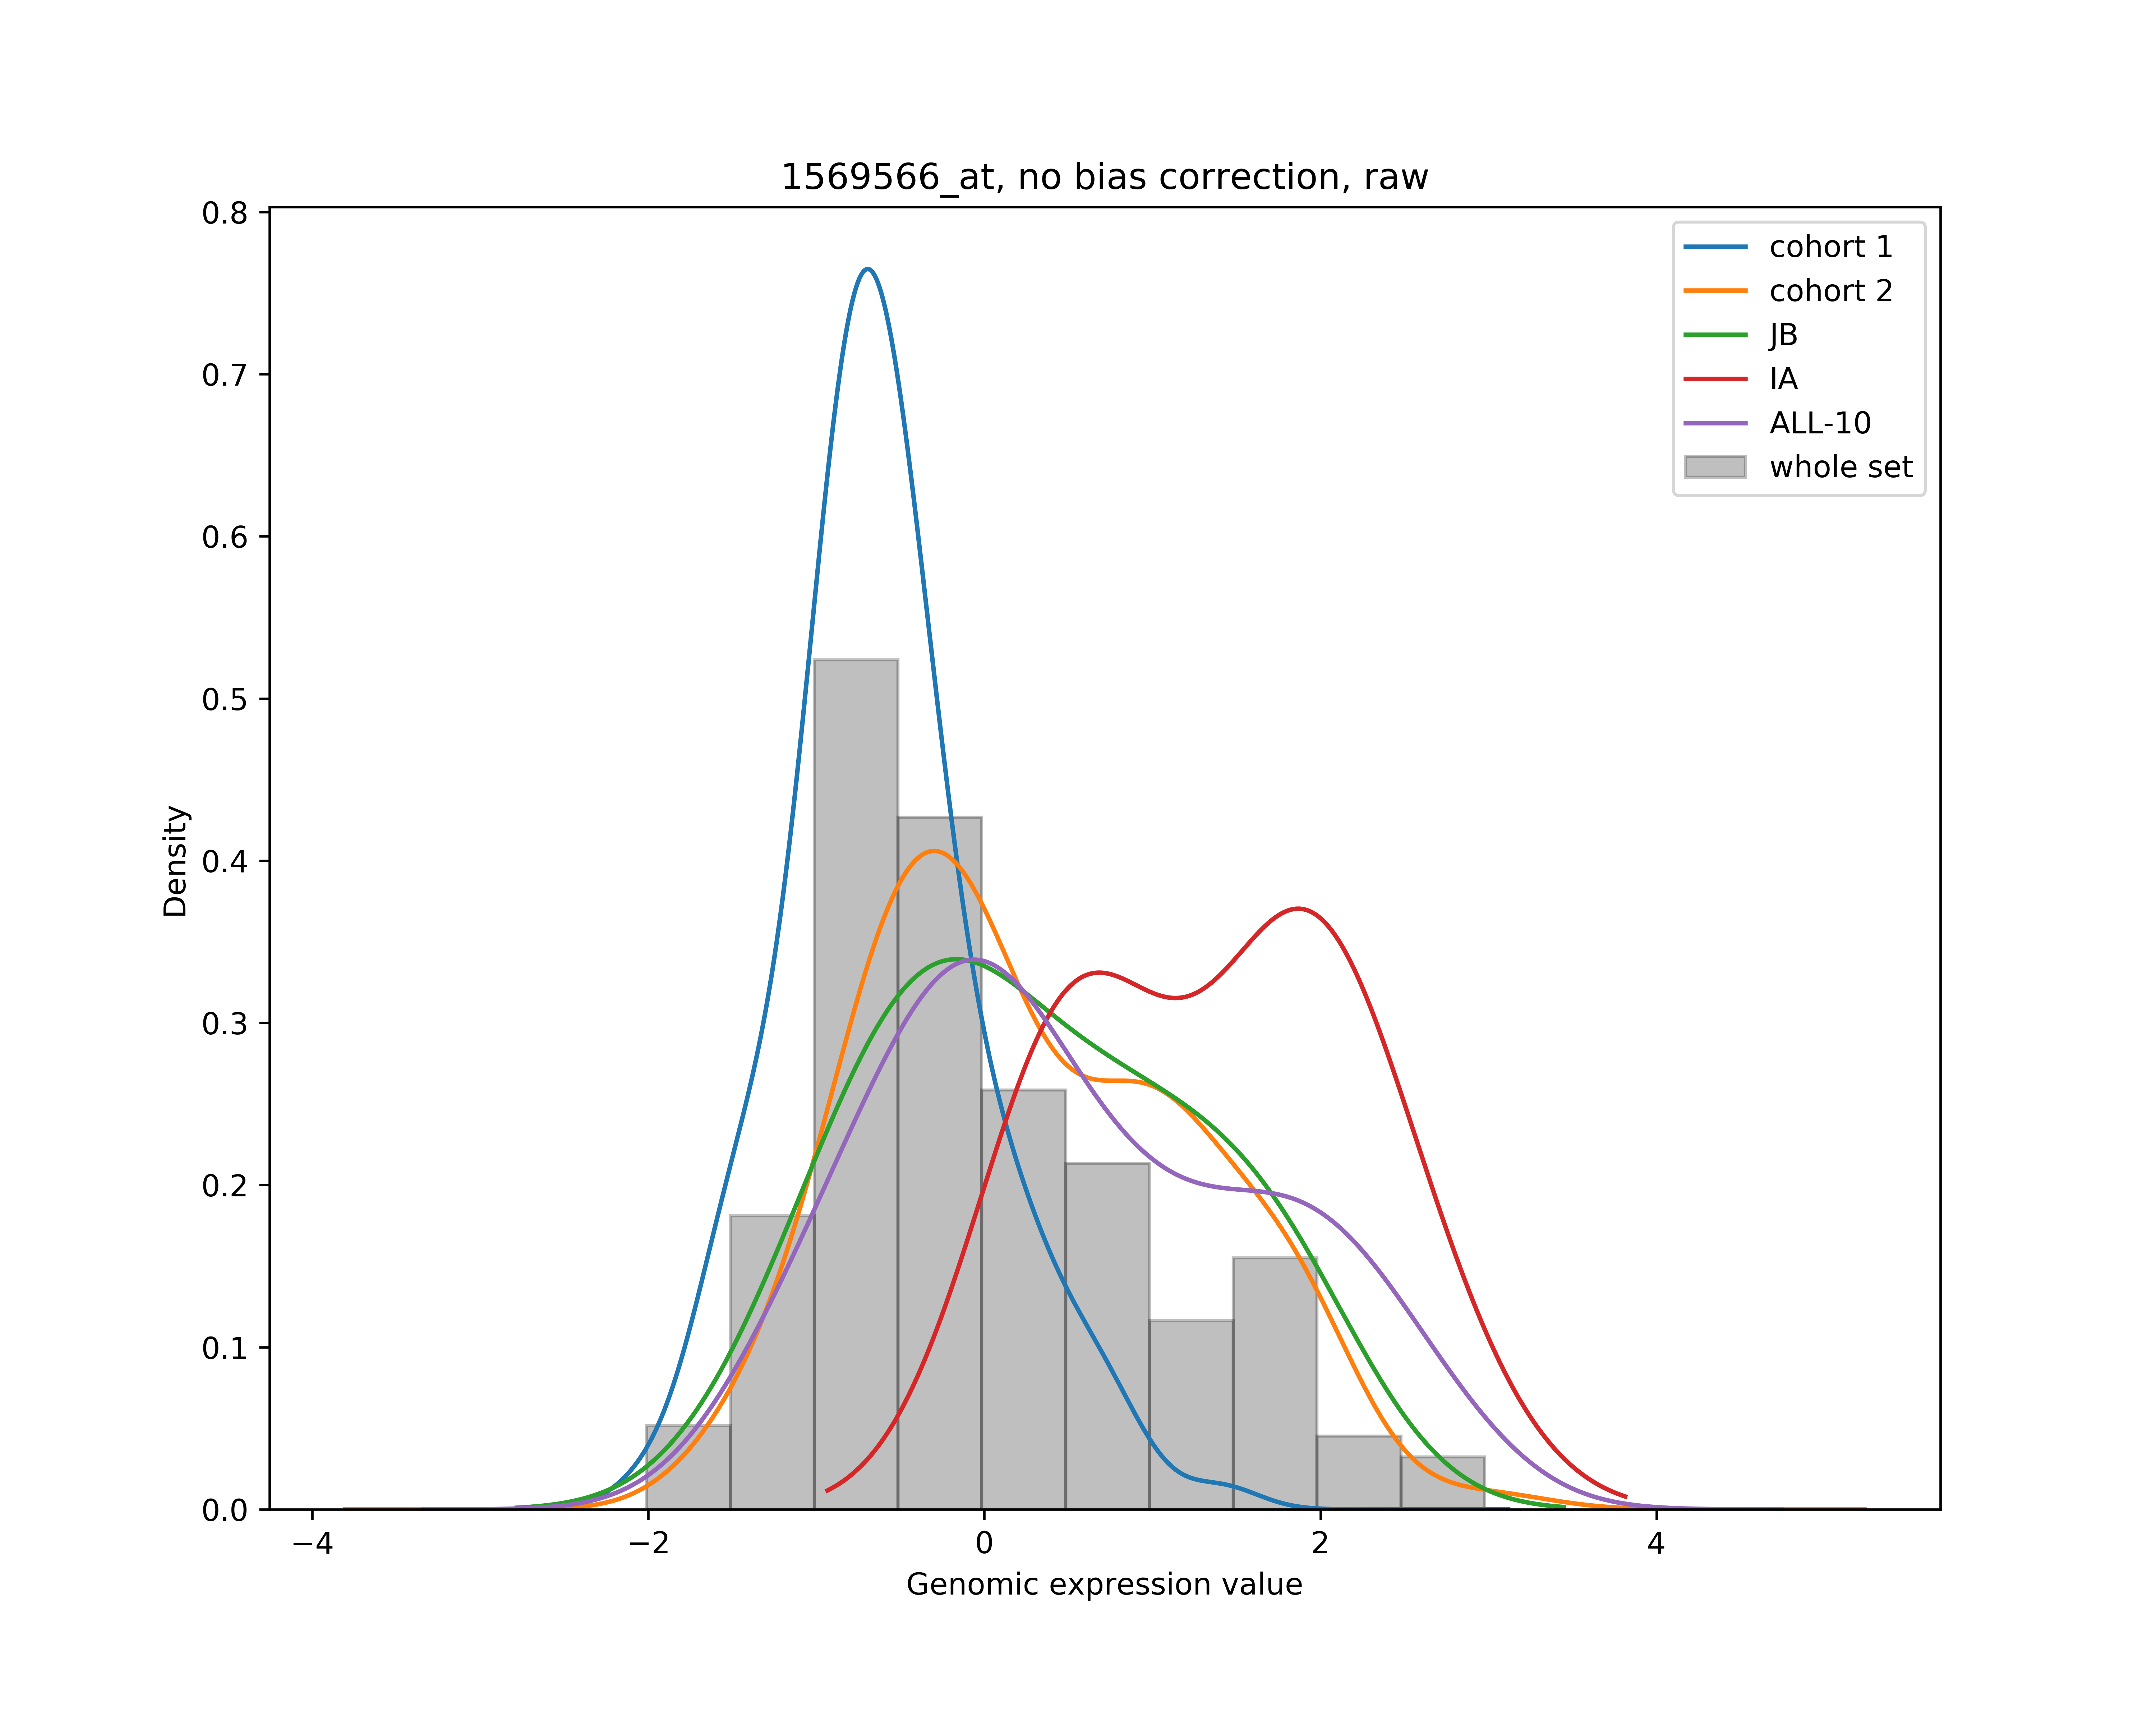
\includegraphics[width=6cm]{images/strong_genome_distribution_noCorrection_noNormalisation}
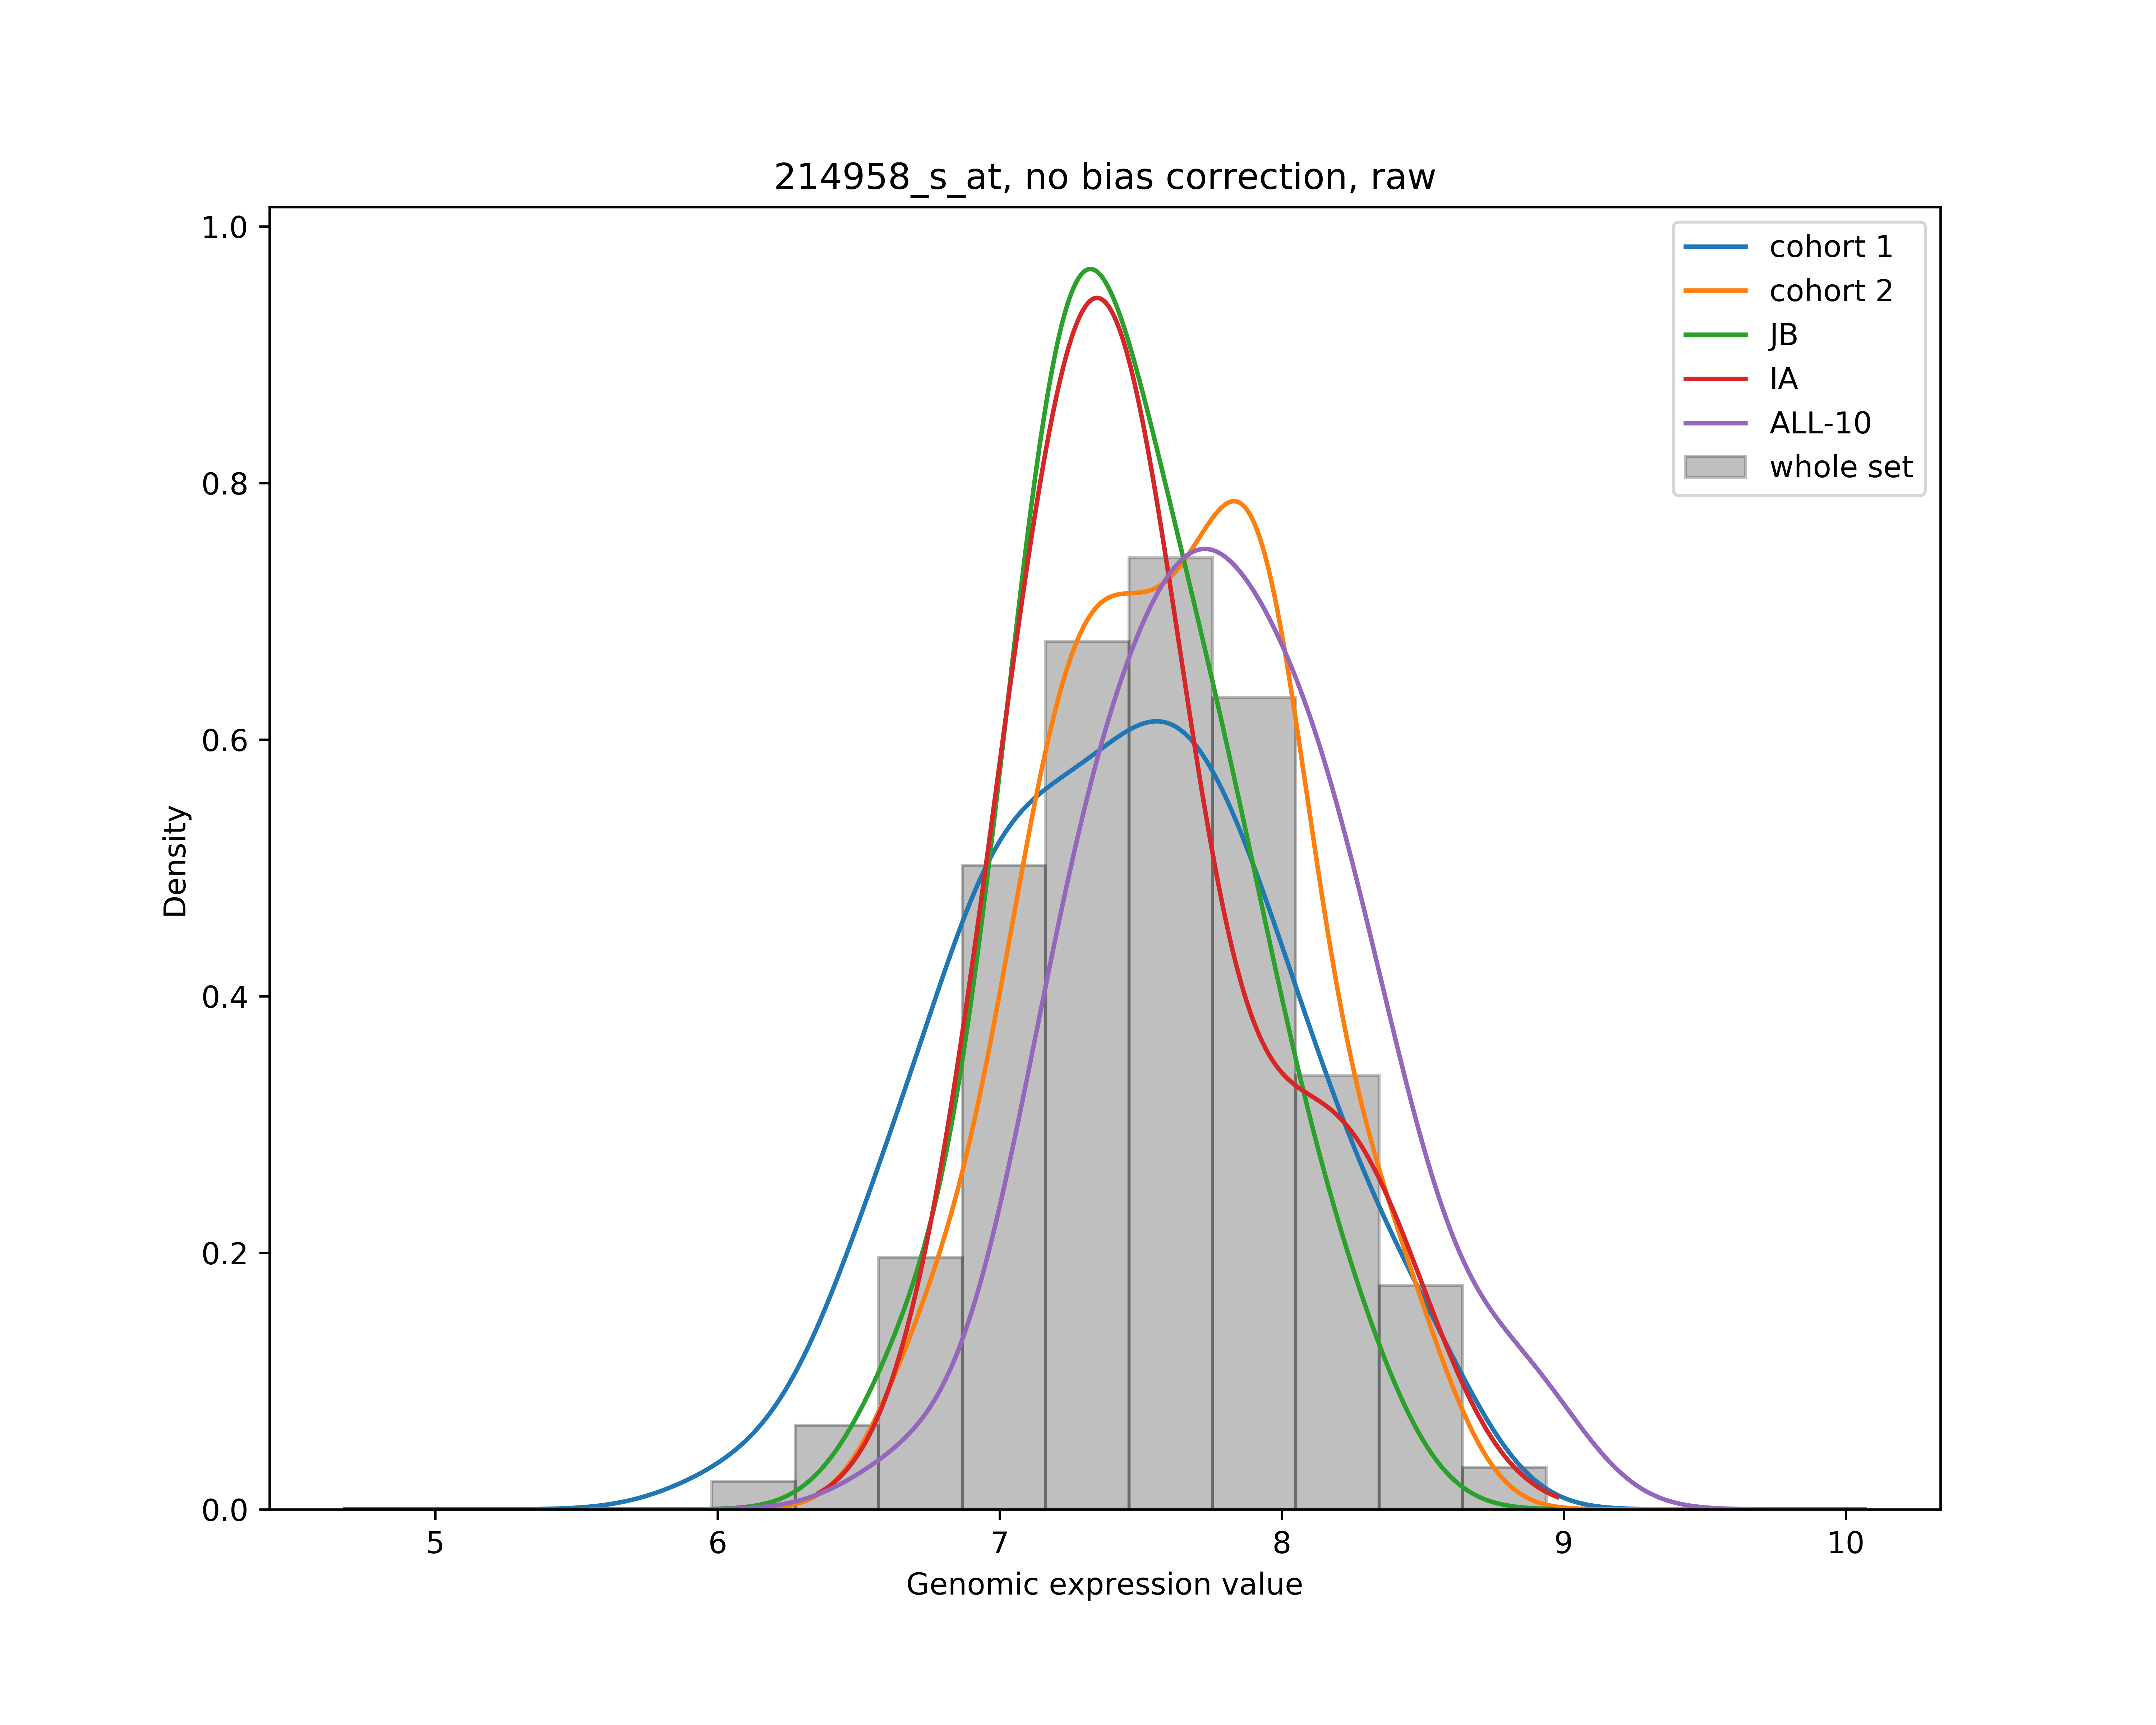
\includegraphics[width=6cm]{images/weak_genome_distribution_noCorrection_noNormalisation}
\caption{Two sets of distributions prior the bias correct, for, (left) a strong predictor and (right) a weak predictor}
\label{fig:expression_distribution_cohorts}
\end{figure}
%
\begin{figure}[htp]
\centering
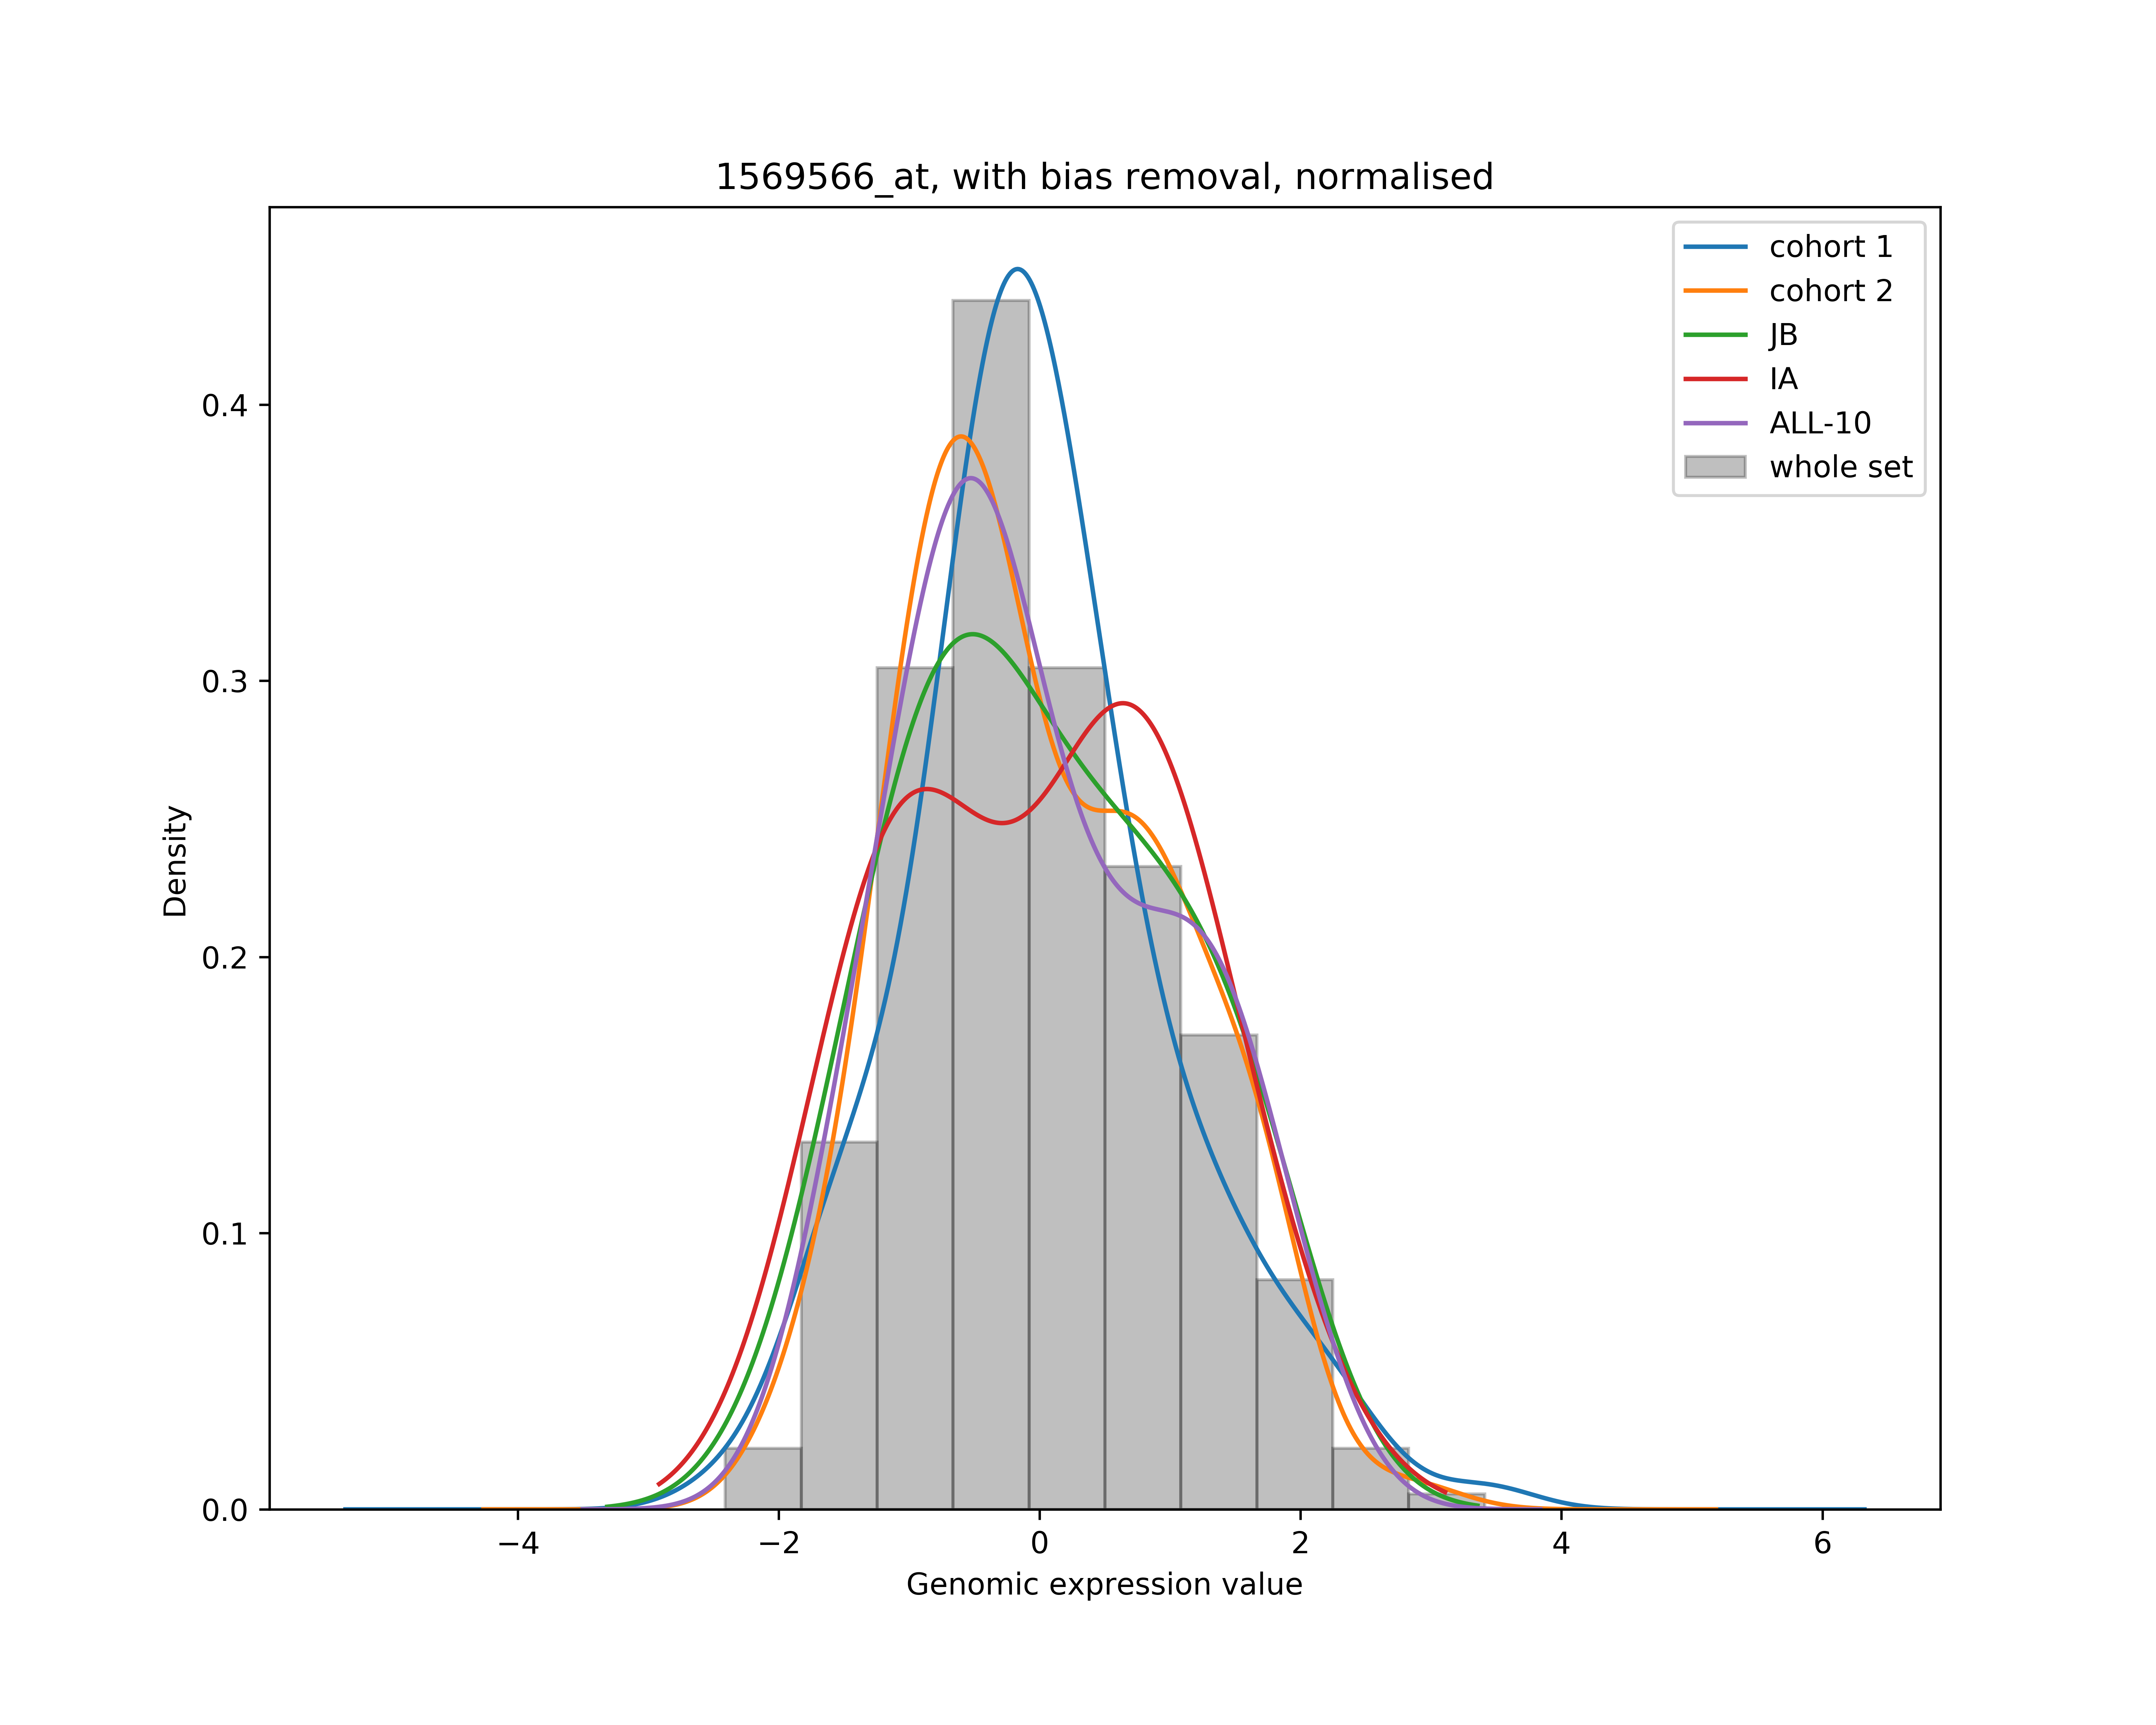
\includegraphics[width=6cm]{images/strong_genome_distribution_withCorrection_standardNormalisation}
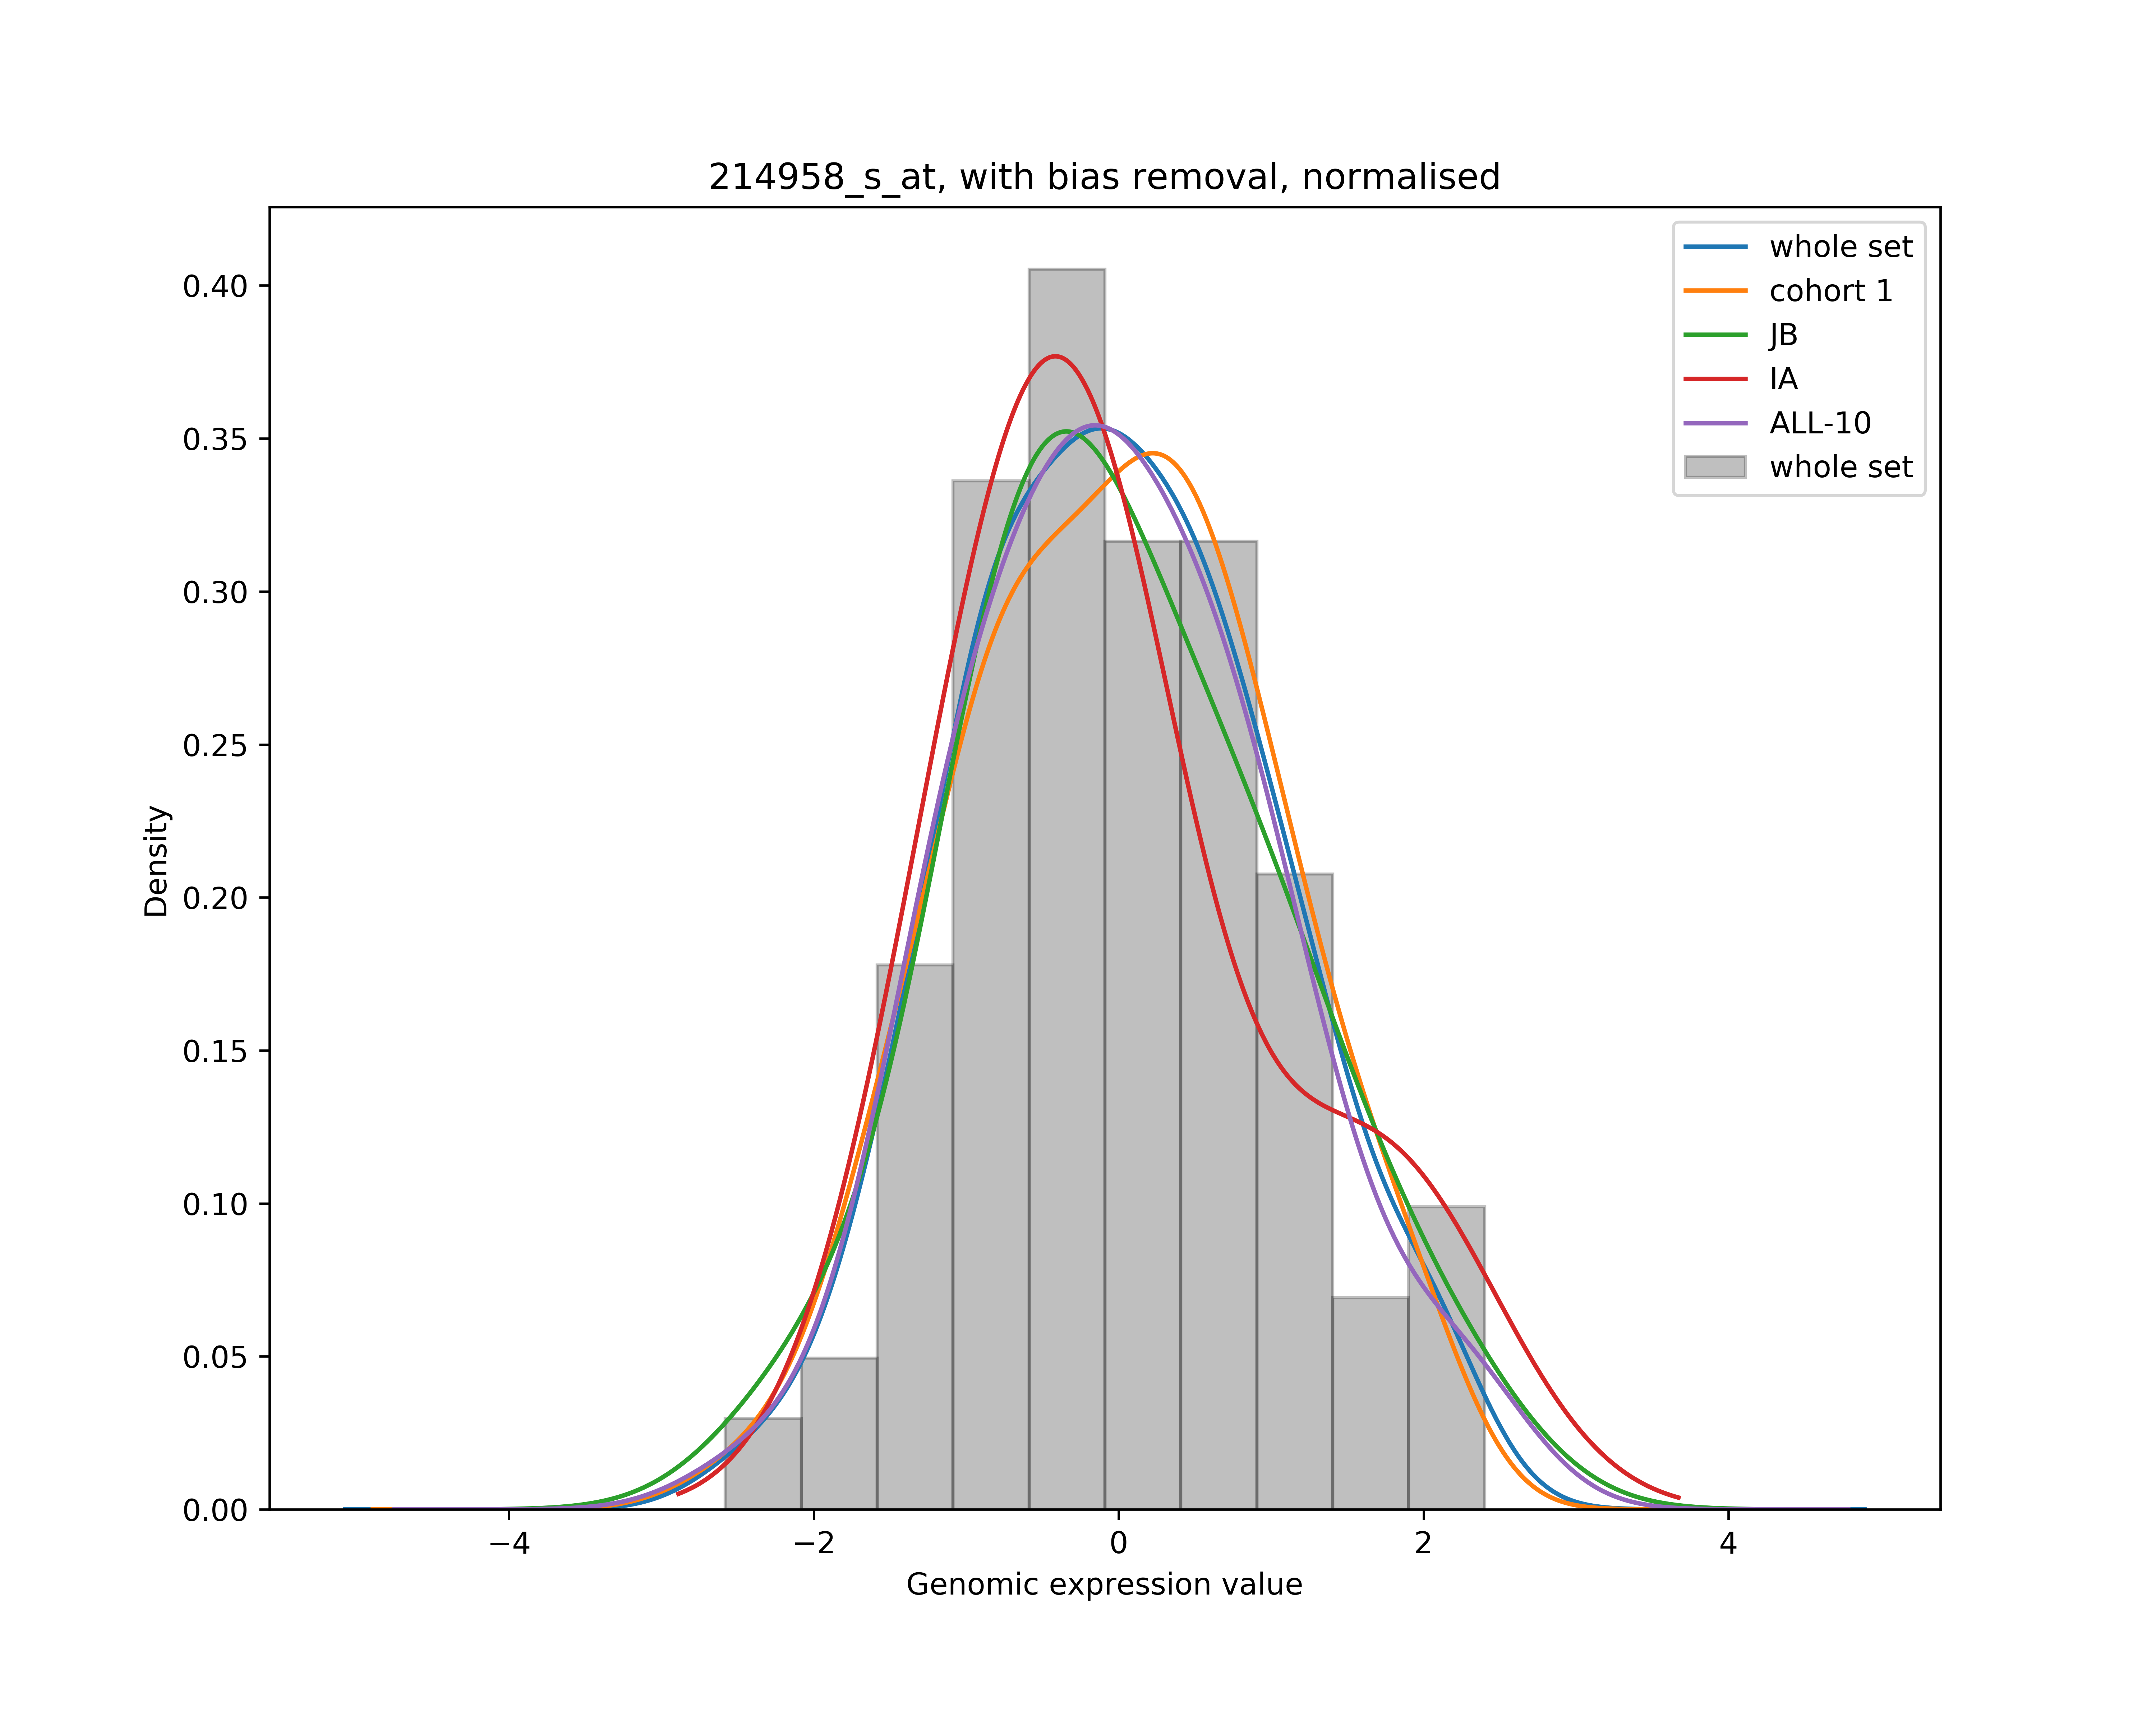
\includegraphics[width=6cm]{images/weak_genome_distribution_withCorrection_standardNormalisation}
\caption{Two sets of distributions with L/S cohort correct, for, (left) a strong predictor and (right) a weak predictor}
\label{fig:expression_distribution_cohorts_withBiasCorrection}
\end{figure}
%Strong: 1569566_at, 223748_at, 223017_at, 1568713_a_at, 201015_s_at
%Weak: 214958_s_at, 200934_at, 207908_at, 205107_s_at, 243806_at
%
There are various more elaborate methods to remove bias such as the SVD-based method from Alter et al.\cite{Alter2000}, the 
PCA-based bias removal methods EIGENSTRAT by Price et al.\cite{Price2006}, MANCIE by Zang et al.\cite{Zang2016}, the distance weighted discrimination (DWD)
approach from Benito et al.\cite{Benito2005} or the ComBat method by Johnson et al.\cite{Johnson2007} who apply an empirical Bayes approach. 
A comparison of bias removal methods is out of scope for this work, for more details we refer the reader to Johnson et al\cite{Johnson2007}.
The basic underlying assumption for all methods is that the samples are stratified over the cohorts, i.e. that in terms
of patients each cohort represents a random selection from the total set of patients. Also, it is assumed that 
the distribution has only one mode. In figures \ref{fig:expression_distribution_cohorts} and \ref{fig:expression_distribution_cohorts_withBiasCorrection}
we show examples of distributions for two different genomes without and with bias removal respectively.

\subsection{Dimension reduction}
%
We considered several dimension reduction techniques such as Principal Component Analysis (PCA, see e.g. Shlens\cite{Shlens2014}), 
Linear Discriminant Analysis (LDA) and the False discovery rate (FDR, see Yoav and Hochberg\cite{Yoav1995}). \\ 
%
PCA is basically a transformation of the feature space based on the eigenvectors 
of the covariance matrix and can be applied to the entire dataset, including the test set.
Using the eigenvectors of the covariance matrix as the basis for the features ensures maximal
variance perpendicular to the coordinate axes. This is a coarse of saying that we maximize the information
content per dimension. The downside is that we obfuscate the biological meaning of the features: any value in the feature set of the transformed matrix is now a linear combination 
of $N$ genome expression values, where $N$ is the number of dimensions. \\
%
In LDA we try to find a linear transformation that maximizes the seperation 
\textbf{between} classes with respect to the seperation \textbf{within} classes, requiring two
covariance matrices. LDA requires availability of the classification label for fitting, hence the transformation is biased to the training set, 
also the features are obfuscated similar to PCA. For both LDA and PCA we need to select the number of dimensions a priori. \\ 
%
The FDR method is basically a feature selection based on a minimum statistical seperarability of the distributions over the different classes.
This minimum seperability is in this case the $p$-value for the rejection of the null hypothesis that the samples are drawn from the same distribution.  \\ 
%
Because the Covariance or linear-discrimination based transformation obfuscates the biological meaning of the feature vectors
we choose the FDR method as the most suitable method to reduce the number of dimensions. Also, the FDR method is commonly applied in genomic research. \\
We apply the FDR method with the Benjamin-Hochberg approach and the ANOVA model to compare the distributions with a maximum $p$-value set at $0.05$. \\ % ANOVA versus Wilcoxon, Mann-Whitney U
%
Arguably, a shortcoming of the FDR method is that, as for LDA, it has a bias towards the training set because it dismisses features solely
on the basis of variance across the different classifications which are obviously not available for the test set. Another shortcoming is that it ignores
feature interdependency, i.e. we may accidentally dismiss feature combinations as predictors because we have removed their constitutive parts. \\ 
%
For this reason, the use of a generic dimension reduction technique such as PCA is advised to improve
the robustness of the model in terms of classification accuracy. As we are currently primarily interested in the importance of individual genomes and not per se the accuracy of the predictor
we consider this out of scope.
%
%
\section{Classification}
%
We will shortly describe the methods used for the predictions and the determination of genome importances.
We will not go in detail on the selection of the method parameters, we refer the reader to the appendix for the
parameter selection.

\subsection{Tree based}

Single decision trees are known to be sensitive to changes in the input data. These ensemble methods 
help to decrease the variance without increasing the bias, i.e. increasing the ability to be generalised.
We employ several tree-ensemble methods: Random Forest (RF) by Breiman\cite{Breiman2001}, ExtraTrees (ET) by Geurts et al.\cite{Geurts2006} 
XGBoost (XGB) by Chen and Guestrin\cite{Chen2016} and (Light)GBM (LGBM) by Ke et al.\cite{Ke2017}.
The RF and ET methods are ensemble methods that combine an arbitrary number of decision trees, using bootstrapped samples,
random feature selection and a majority vote classification. The XGB and LGBM methods are ensemble methods 
that apply a technique called gradient boosting by Breiman\cite{Breiman1997}.
%
\subsection{Neural networks}
%
We use $2$ types of neural networks, a Deep Neural Network (DNN) \cite{lecun2015deep} and a Convolutional Neural Network (CNN) \cite{Lecun98}. The main advantage of neural networks is that they can learn nonlinear relationships between features. Despite the small sample size, it is interesting to apply neural networks in this context due to the high dimensionality of the data. Neural networks with multiple layers are proficient in discerning more subtle patterns in the data compared to other approaches. Shallow neural networks have been succesfully applied to similar sets of genetic expression data in the past, such as in \cite{khan2001classification}.
A DNN, as shown in figure \ref{fig:dnn_architecture}, uses several fully connected layers of nodes as a network architecture. A high level explanation of the difference between DNNs and CNNs is that a DNN looks at the entire dataset in each node (layers are fully connected).
While a CNN contains operations that allow it to focus on smaller subsets of the data (convolutional layers) 
and operations that allow it to filter out irrelevant data (pooling layers). An example of a CNN architecture for image classification is shown in figure \ref{fig:cnn_architecture}.

\begin{figure}[htp]
  \centering{}
  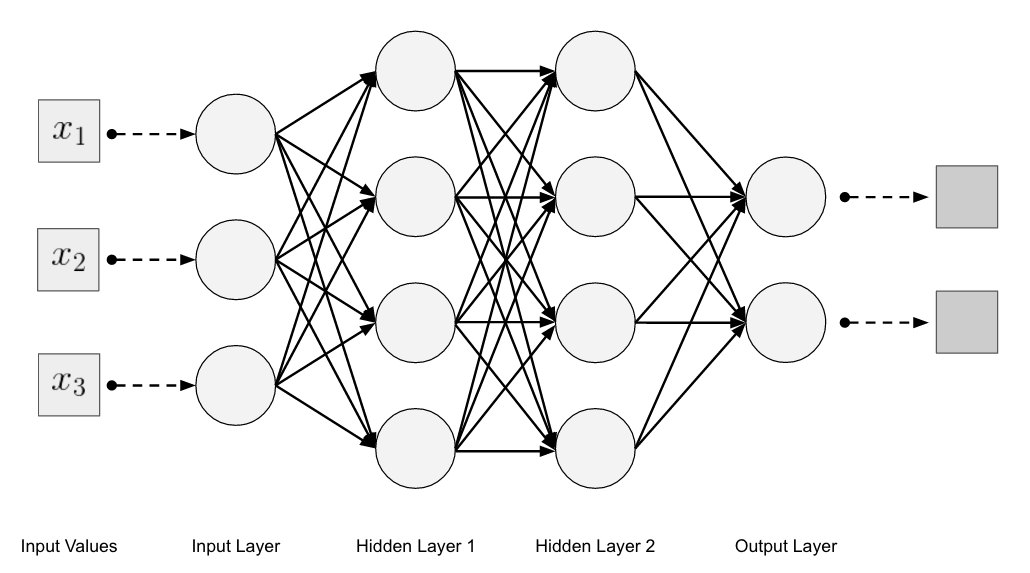
\includegraphics[width=8cm]{images/DNN}
  \caption{A generic architecture for a deep feedforward neural network.}
  \label{fig:dnn_architecture}
\end{figure}

\begin{figure}[htp]
  \centering
  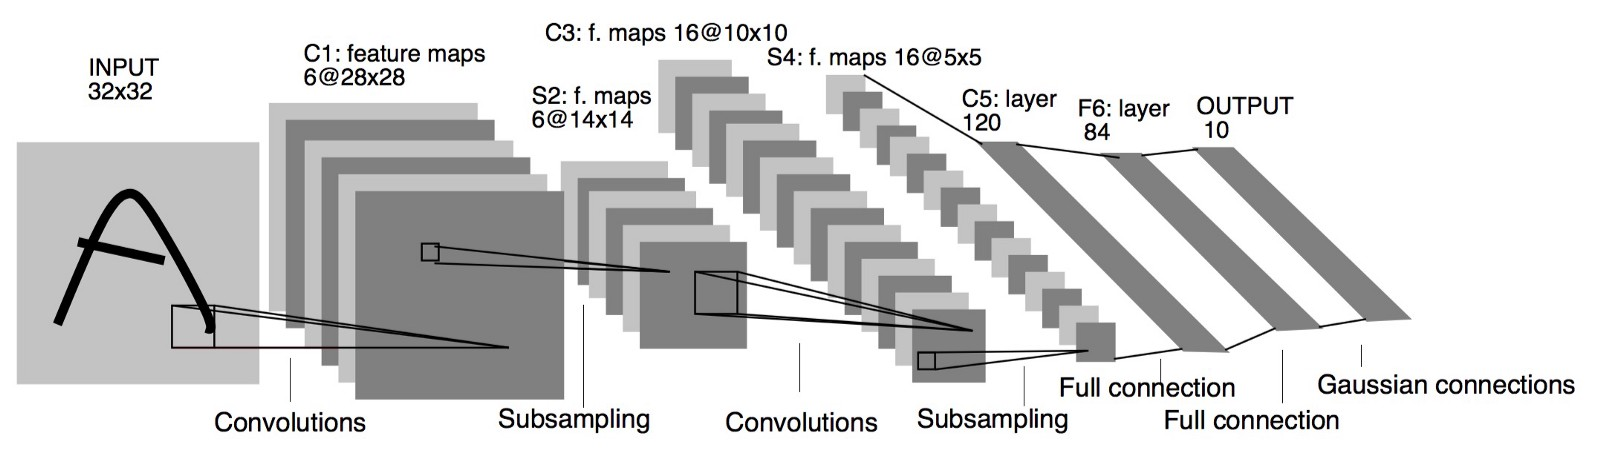
\includegraphics[width=8cm]{images/CNN}
  \caption{A typical convolutional neural network architecture for image classification from \cite{Lecun98}.}
  \label{fig:cnn_architecture}
\end{figure}

It is not possible out-of-the-box to discern which features are important for the final prediction. 
Using Local Interpretable Model-Agnostic Explanations (LIME) developed by Ribeiro et al.\cite{Ribeiro2016} 
we can get an idea of the so-called local decision boundary for individual samples which may assist in
understanding the model decision in that particular case but I cannot 
%
\subsection{Linear methods}

Logistic Regression (LR), 
linear Support Vector Machines (lSVM), 
linear discriminant analysis (LDA)

Simplicity, transparancy, robustness. However, what we gain in expressiveness we may lose in accuracy.

\subsection{Probabilistic methods}
%
Naive Bayes (NB), Gaussian Processes (GPC), Relevance Vector Machines (RVM)


\section{Results}
% 
\begin{table}[htp]
\centering
\caption{Mean accuracies over $10$ runs with $1\%$ added random noise per run}
\label{tab:diversitymetrics}
\begin{tabular}{lllllll}
				& RF     & DNN 		& CNN  		& LSVM 		& 	XGB 	& 	LDA  \\
FDR $\alpha=0.05$		& 0.38   &  0.29      	&  0.38     	&  0.43    	& 0.25    	& 0.42  \\
FDR $\alpha=0.1$ 		& 1.59   &  1.70      	&  1.68 	&  1.65    	& 1.79    	& 1.66  \\
PCA $N=200$    			& 1.86   &  2.10      	&  1.88         &  1.79    	& 1.88          & 1.76  \\
LDA $N=200$        		& 1.54   &  1.73      	&  1.65         &  1.56    	& 1.48          & 1.55  \\
PCA $N=500$    			& 1.86   &  2.10      	&  1.88         &  1.79    	& 1.88          & 1.76  \\
LDA $N=500$        		& 1.54   &  1.73      	&  1.65         &  1.56    	& 1.48          & 1.55  \\
\end{tabular}
% Why is the mean accuracy not between 0 and 1? Are these placeholder results?
\end{table}
%

The tree-methods are not sensitive to the bias removal, or to the normalisation.
% Is this correct? Seperate bias removal for each cohort might change the overall ordering of a feature -> which does make a tree sensitive to bias removal
% good point: it could also be that the tree methods mostly ignore the weak features automagically but I will need to verify.
% Tree methods do their own feature selection, if it is not possible to make a decent split of the data with a certain feature itll be ignored, however since the sample size is so small it still might be able to make a decent split on a shit feature, because of pure luck. I was talking about the bias removal tho, which doesn't have much to do with feature selection?
\section{Post-processing}
%
Description of weight/importance retrieval

\section{Discussion}

\begin{itemize}
\item if we choose PCA, LDA, check for inflection point in eigenvalue magnitude to 'smartly' select the number of components
\item successively apply standard scaling and maxabs scaling to center cohort data?
\item improve bias removal method L/S by ignoring outliers during normalisation
\item we can combine the different models in one meta-model. This bagging of models increases the accuracy, removes method-specific biases and at the same time its helps reduce overfitting.
The downside of bagging is that it obfuscates the results.
\end{itemize}

\bibliographystyle{plain}
\bibliography{methods}
\end{document}
